\documentclass[12pt]{article}
\usepackage[utf8]{inputenc}
\usepackage{array}
\newcolumntype{C}[1]{>{\centering\let\newline\\\arraybackslash\hspace{0pt}}m{#1}}
\usepackage[spanish]{babel}
 \usepackage{url}
\usepackage[spanish, fixlanguage]{babelbib}
\bibliographystyle{IEEEtran}
\usepackage{graphicx}
\graphicspath{ {./images/} }
\usepackage{amssymb}
\usepackage{amsmath}
\usepackage{subcaption}
\usepackage[linesnumbered]{algorithm2e}
\newcommand\mycommfont[1]{\footnotesize\ttfamily\textcolor{blue}{#1}}
\SetCommentSty{mycommfont}
\usepackage{tikz}
\usetikzlibrary{positioning, fit}
\usetikzlibrary{babel}
\usepackage{titlesec}
\titlespacing*{\section}
{0pt}{5.5ex plus 1ex minus .2ex}{.3ex plus .1ex}
\titlespacing*{\subsection}
{0pt}{5.5ex plus 1ex minus .2ex}{2.3ex plus .1ex}

\title{Tarea 4}

\author{
	Saul Ivan Rivas Vega \\
	\\
	Diseño y análisis de algoritmos\\
\\
	Equipo Completo:\\
		Yadira Fleitas Toranzo\\
		Diego de Jesús Isla Lopez\\
		Saul Ivan Rivas Vega\\
}

\date{\today}

\begin{document}
	\maketitle
	\pagebreak
	\section{Ejercicio 1.}
	\subsection{Da un ejemplo de una familia de digráficas de $n$ vértices con pesos no negativos tal que admita una ejecución del algoritmo de Dijkstra en la cual todos los nodos actualizan a su padre y su estimación de distancia $d(v)$ una sola vez; es decir, la primera oferta de camino que reciben, es la del camino mas corto. Demuestra que tu ejemplo cumple lo que se pide.}
	\paragraph{}Sea $F$ la familia de digráficas que cumpla las siguientes condiciones para cada miembro $G$ de ella:\\
	\begin{itemize}
		\item La gráfica $G$ tiene un conjunto de aristas ponderadas $E$ tal que $|E| = n$ donde cada arista tiene un peso mayor o igual a cero y un conjunto de vértices $V$ tal que $|V| = n$.
		\item $G$ es conexa.
		\item Todo $v\in V$ tiene $inDegree(v) = 1$, es decir que tienen exactamente una sola arista de entrada.
		\item Todo $v\in V$ tiene $outDegree(v) = 1$, es decir que tienen exactamente una sola arista de salida. 
		\item Solo hay un ciclo y todo $v\in V$ esta en el ciclo.
	\end{itemize}
	Un miembro de esta familia con $n=6$ es:\\
	\begin{center}
	\begin{tikzpicture}[roundnode/.style={draw,shape=circle,fill=black!40,minimum size=1mm}]
		\tikz
		%Nodes
		\node[roundnode,label={north west:$v_1$}]      (v1)                     {};
		\node[roundnode,label={north east:$v_2$}]      (v2)       [right=of v1] {};
		\node[roundnode,label={east:$v_3$}]      (v3)       [below right=of v2] {};
		\node[roundnode,label={south east:$v_4$}]      (v4)       [below left =of v3] {};
		\node[roundnode,label={south west:$v_5$}]      (v5)       [left =of v4] {};
		\node[roundnode, label={west:$v_6$}]      (v6)       [below left =of v1] {};
		%Lines
		\draw[->] (v1) -- (v2) node[midway,below] {2};
		\draw[->] (v2) -- (v3) node[midway,below] {4};
		\draw[->] (v3) -- (v4) node[midway,below] {1};
		\draw[->] (v4) -- (v5) node[midway,below] {4};
		\draw[->] (v5) -- (v6) node[midway,below] {0};
		\draw[->] (v6) -- (v1) node[midway,below] {5}; 
	\end{tikzpicture}
	\end{center}
	\paragraph{Demostración} Por contradicción.\\
	Supongamos que durante una ejecución el algoritmo de Dijkstra al empezar en cualquier nodo $s\in G$, existe un nodo $v_i$ tal que $v_i \neq s$ y además actualizó su estimación de distancia $d(v_i)$ mas de una vez.\\
	Entonces el algoritmo hizo una primera estimación de distancia $d(v_i)_1$ siguiendo un camino de nodos $p$ desde $s$ hasta $v_i$. Ahora para realizar una estimación adicional $d(v_i)_2$ tal que $d(v_i)_2 < d(v_i)_1$ debió encontrar un segundo camino $p'$ para llegar a $v_i$.\\
	Sin embargo, siendo $G$  miembro de la familia $F$ se cumple que todo $v\in G$ tiene una sola arista de salida y una de entrada, y solo hay un ciclo donde todo $v\in G$ esta en el. Le sigue que, para llegar a $v_i$ desde $s$, se puede:
	\begin{enumerate}
		\item Seguir el ciclo hasta llegar a $v_i$.
		\item Completar el ciclo $z$ veces ($z>=1$) y volver a llegar a $v_i$.
	\end{enumerate}  
	El camino resultante de al usar el segundo método será siempre mayor o igual al primero puesto que los pesos son mayores o iguales a 0 manteniendo o incrementando el camino del primer método.\\
	Por lo tanto existe un solo camino mínimo entre cualquier par de nodos en $G$. Entonces no existe un segundo camino $p'$ tal que al llegar a $v_i$ su estimación de distancia cumpla que $d(v_i)_2 < d(v_i)_1$ y en la ejecución no hubo una actualización adicional a la primera, pero esto es una contradicción a nuestra suposición inicial. Finalmente, en cualquier ejecución del algoritmo empezando en cualquier nodo $s\in G$, todos los nodos actualizan a su padre y su estimación de distancia $d(v_i)$ una sola vez.
	\pagebreak
	\subsection{Da un ejemplo de una familia de digráficas con pesos no negativos tal que cualquier ejecución del algoritmo de Dijkstra requiera que algún vértice actualice su padre y su estimación de distancia dos veces. Demuestra que tu ejemplo cumple lo que se pide.}
		\paragraph{}Sea $F$ la familia de digráficas que cumpla las siguientes condiciones para cada miembro $G$ de ella:\\
	\begin{enumerate}
		\item Tiene un nodo inicial $s$ el cual no tiene aristas de entrada.
		\item $s$ tiene una arista de salida con peso igual a 1.
		\item Tiene un nodo final $v_f$ el cual no tiene aristas de salida.
    	\item $v_f$ tiene una arista de entrada con peso igual a 1.
		\item Para todo $v\in G$ tal que $v\neq s$ y $v\neq v_f$, se cumple:
			\begin{enumerate}
				\item $v$ tiene una sola arista de entrada con peso igual a 1.
				\item $v$ tiene una sola arista de salida con peso igual a 1.
			\end{enumerate}
	\item Desde $s$ se puede llegar a todos los otros vértices.
	\item Hay una arista adicional desde $s$ a $v_f$ con peso $2n$.
	\item $s$ tiene exactamente 2 aristas de salida.
	\item $v_f$ tiene exactamente 2 aristas de entrada.
	\end{enumerate}
	Un miembro de esta familia con $n=4$, donde $s = v_1$ y $v_f = v_4$ es:\\
	\begin{center}
		\begin{tikzpicture}[roundnode/.style={draw,shape=circle,fill=black!40,minimum size=1mm}]
		\tikz
		%Nodes
		\node[roundnode,label={north west:$v_1$}]      (v1)                     {};
		\node[roundnode,label={north west:$v_2$}]      (v2)       [right=of v1] {};
		\node[roundnode,label={north west:$v_3$}]      (v3)       [right=of v2] {};
		\node[roundnode,label={north west:$v_4$}]      (v4)       [right =of v3] {};
		%Lines
		\draw[->] (v1) -- (v2) node[midway,below] {1};
		\draw[->] (v2) -- (v3) node[midway,below] {1};
		\draw[->] (v3) -- (v4) node[midway,below] {1};
		\draw[->] (v1) to [out=270,in=240] node[pos=0.5, below] {8}  (v4) ;
		\end{tikzpicture}
	\end{center}
	\paragraph{Demostración} Propongamos al vértice $v_f$ como aquel nodo que actualice su padre y su estimación de distancia dos veces al comenzar desde el nodo $s$.\\
	La primer estimación de distancia $d(v_f)_1$se realiza al ejecutar el algoritmo iniciando en $s$, pues $v_f$ es vecino directo por la propiedad $7$. $d(v_f)_1$ vale $2n$. Ahora para una segunda estimación se puede seguir el camino de la otra arista de peso 1 de  $s$, dicho camino llegará a $v_f$ por  la propiedad $6$. \\ Este camino tendrá como peso total la suma de los pesos de las aristas, cada arista en ese camino tiene peso 1, y como pasa por todos los nodos y todos menos $v_f$ tienen una arista de salida de peso 1, significa que hay $n-1$ aristas. Posteriormente tenemos que esta segunda estimación $d(v_f)_2$ vale $n-1$. Finalmente como $d(v_f)_2  < d(v_f)_1$ habrá forzosamente una segunda actualización.
	\section{Ejercicio 2.}
	\subsection{De acuerdo con el algoritmo de Dijkstra que revisamos en clase, para cada $n\in \mathbb{N}$ con $n>2$, presenta una familia de gráficas de $n$ vértices con pesos tanto positivos como negativos y sin ciclos dirigidos de longitud negativa para la cual se cumple que si $G$ es una gráfica de la familia, el algoritmo de Dijkstra falla en encontrar el camino más corto entre $s$ y algún otro vértice de $G$. Demuestra que de hecho existe tal vértice.}
	\paragraph{}Sea $F$ la familia de digráficas que sigue el siguiente proceso de construcción:\\
	Para $G_0$ se tiene la siguiente gráfica:
		\begin{center}
			\begin{tikzpicture}[roundnode/.style={draw,shape=circle,fill=black!40,minimum size=1mm}]
			\tikz
			%Nodes
			\node[roundnode,label={north west:$v_1$}]      (v1)                     {};
			\node[roundnode,label={north west:$v_2$}]      (v2)       [above right=of v1] {};
			\node[roundnode,label={north east:$v_3$}]      (v3)       [below right=of v2] {};
			%Lines
			\draw[->] (v1) -- (v2) node[midway,above] {$z$};
			\draw[->] (v2) -- (v3) node[midway,above] {$-z$};
			\draw[->] (v1) -- (v3) node[midway,below] {1};
			\end{tikzpicture}
		\end{center}
		Donde $z = 2n$, en $G_0$ $z=6$.\\
		Ahora para cualquier otro $G_i$ con $i>0$ se agregará una arista del último nodo de $G_{i-1}$, el cual es $v_{i+2}$, a un nuevo nodo $v_{i + 3}$ con peso 1: 
				\begin{center}
			\begin{tikzpicture}[roundnode/.style={draw,shape=circle,fill=black!40,minimum size=1mm}]
			\tikz
			%Nodes
			\node[roundnode,label={north west:$v_1$}]      (v1)                     {};
			\node[roundnode,label={north west:$v_2$}]      (v2)       [above right=of v1] {};
			\node[roundnode,label={north east:$v_3$}]      (v3)       [below right=of v2] {};
			\node[label={$...$}]      (v4)       [right=of v3] {};
			\node[roundnode,label={north east:$v_{i+2}$}]      (v5)       [right=of v4] {};
    		\node[roundnode,label={north east:$v_{i+3}$}]      (v6)       [right=of v5] {};
			%Lines
			\draw[->] (v1) -- (v2) node[midway,above] {$z$};
			\draw[->] (v2) -- (v3) node[midway,above] {$-z$};
			\draw[->] (v1) -- (v3) node[midway,below] {1};
			\draw[->] (v3) -- (v4) node[midway,below] {1};
			\draw[->] (v4) -- (v5) node[midway,below] {1};
    		\draw[->] (v5) -- (v6) node[midway,below] {1};
			\end{tikzpicture}
		\end{center}
	\paragraph{Demostración} La ejecución de Dijkstra empieza en $v_1$ y propongamos que donde falla en encontrar el camino mínimo es para el nodo $v_3$.\\
	En la primera ocasión donde se estiman distancias a partir de $v_1$ se marca como explorados a $v_2$ y a $v_3$.
	La estimaciones son: $d(v_2)=z$ y $d(v_3)=1$. Esas son las primeras estimaciones para cualquier ejecución del algoritmo con nodo inicial en $v_1$.\\
	Ahora como $z=2n$ y $2n>1$ el algoritmo seguirá explorando ahora con $v_3$. Solo se consideraría ir por $v_2$ cuando la estimación de distancia para algún nodo $v_i$ cumpla que $d(v_i) > 2n$, sin embargo como las aristas tienen peso 1, y no hay mas de $n-3$ aristas a partir de $v_3$, nunca se considerará explorar a partir de $v_2$.\\
	Por lo tanto al explorar todos los nodos se terminará la ejecución del algoritmo y la estimación de distancia para $v_3$ es $d(v_3)=1$, sin embargo al tomar el camino de $v_1$ a $v_2$ y luego a $v_3$ se tendría una distancia de $0$, la cual es menor a $1$. Finalmente para cualquier gráfica $G$ miembro de la familia al ejecutar el algoritmo de Dijkstra empezando en $v_1$, el algoritmo fallará en encontrar la distancia mínima para el nodo $v_3$.
	\subsection{Toma una gráfica de la familia que propones y muestra que Bellman-Ford si encuentra el camino que Dijkstra no.}
	Tomemos a $G_0$:
	\begin{center}
		\begin{tikzpicture}[roundnode/.style={draw,shape=circle,fill=black!40,minimum size=1mm}]
		\tikz
		%Nodes
		\node[roundnode,label={north west:$v_1$}]      (v1)                     {};
		\node[roundnode,label={north west:$v_2$}]      (v2)       [above right=of v1] {};
		\node[roundnode,label={north east:$v_3$}]      (v3)       [below right=of v2] {};
		%Lines
		\draw[->] (v1) -- (v2) node[midway,above] {$6$};
		\draw[->] (v2) -- (v3) node[midway,above] {$-6$};
		\draw[->] (v1) -- (v3) node[midway,below] {1};
		\end{tikzpicture}
	\end{center}
	\begin{algorithm}[H]\footnotesize
	\SetAlgoLined
	Inicializar $d(v)=infinito$, para toda $v \in G$\;
	Asignar $d(s)=0$\;
	\For{i desde 1 hasta (n-1)}{
		\ForEach{Arista $(u,v,peso) \in E$}{ 
				\If{$d(u) + peso < d(v)$}{\emph{$d(v) := d(u) + peso$}\;}
		}
	}
	\caption{Bellman-Ford.}
	\end{algorithm}
	\paragraph{Demostración} Sea $v_1$ el nodo $s$ para el algoritmo.\\
	Al inicializar las distancias como en las lineas 1 y 2 tenemos:
	\begin{itemize}
		\item $d(v_1)=0$. 
		\item $d(v_2)=infinito$.
		\item $d(v_3)=infinito$.
	\end{itemize}
	En la primera ejecución del ciclo en la linea 3 se prueban las siguientes aristas con las correspondientes evaluaciones:
	\begin{itemize}
		\item Arista$(v_1, v_2, 6)$.
		\begin{itemize}
				\item $d(v_1) + 6 < d(v_2)$.
				\item $0 + 6 < infinito$.
				\item true. Asignamos $d(v_2) := 6$
			\end{itemize}
	\item La arista $(v_1, v_3, 1)$ pudo haber sido evaluada en dos casos:
	\begin{enumerate}
		\item Cuando $d(v_3)=infinito - 6$, es decir evaluamos primero a la arista $(v_2, v_3, -6)$.
		\begin{itemize}
			\item $d(v_1) + 1 < d(v_3)$.
			\item $1 < infinito-6$.
			\item true. Asignamos $d(v_3) := 1$
		\end{itemize}
		\item Cuando $d(v_3)=infinito$, es decir todavía no evaluamos a la arista $(v_2, v_3, -6)$.
		\begin{itemize}
			\item $d(v_1) + 1 < d(v_3)$.
			\item $0 + 1 < infinito$.
			\item true. Asignamos $d(v_3) := 1$
		\end{itemize}
		
	\end{enumerate}
		\item La arista $(v_2, v_3, -6)$ pudo haber sido evaluada en los mismos dos casos:
		\begin{enumerate}
			 \item Cuando $d(v_2)=infinito$, es decir todavía no evaluamos a la arista $(v_1, v_2, 6)$.
			 \begin{itemize}
			 	\item $d(v_2) + (-6) < d(v_3)$.
			 	\item $infinito - 6 < infinito$.
			 	\item true. Asignamos $d(v_3) := infinito - 6$
			 \end{itemize}
			 \item Cuando $d(v_2)=6$, es decir evaluamos primero a la arista $(v_1, v_2, 6)$.
			 \begin{itemize}
			 	\item $d(v_2) + (-6) < d(v_3)$.
			 	\item $6 - 6 < infinito$.
			 	\item true. Asignamos $d(v_3) := 0$
			 \end{itemize}
		\end{enumerate}
	\end{itemize}
	De haber sido el caso número 2, la distancia ya es correcta para $v_3$ siendo $d(v_3)=0$, sin embargo esa distancia se alcanza en la segunda iteración para el caso número 1:
	\begin{itemize}
	\item La arista $(v_2, v_3, -6)$ tomando el caso numero 1 de la iteración anterior se realiza la siguiente evaluación:
			\begin{itemize}
				\item $d(v_2) + (-6) < d(v_3)$.
				\item $6 - 6 < 1$.
				\item true. Asignamos $d(v_3) := 0$
			\end{itemize}
	\end{itemize}
Finalmente se asegura que Bellman-Ford llega a la distancia correcta de $v_3$ siendo $d(v_3)=0$, a diferencia de Dijkstra que reportaría erróneamente $d(v_3)=1$ como se muestra en la demostración del ejercicio 2.1.
\section{Ejercicio 3}
\subsection{De acuerdo con el algoritmo de Dijkstra que revisamos en clase, para cada $n\in \mathbb{N}$ con $n>2$, presenta una familia de gráfircas de $n$ vértices con pesos positivos y negativos y sin ciclos dirigidos de longitud negativa para la cual se cumple que si $G$ es una gráfica de la familia, el algoritmo de Dijkstra no falla en encontrar el camino más corto entre dos vértices de $G$. Prueba que en efecto el algoritmo encuentra los caminos más cortos.}
\paragraph{}
	Para $G_0$ se tiene la siguiente gráfica:
\begin{center}
	\begin{tikzpicture}[roundnode/.style={draw,shape=circle,fill=black!40,minimum size=1mm}]
	\tikz
	%Nodes
	\node[roundnode,label={north west:$v_1$}]      (v1)                     {};
	\end{tikzpicture}
\end{center}
Es decir un solo nodo $v_1$. Ahora para cualquier otro $G_i$ con $i>0$ se agregará un nuevo nodo $v_{i+1}$ y una arista de $v_{i} $ a $v_{i+1}$ con peso $w_i$ positivo, negativo o igual a 0. 
\begin{center}
	\begin{tikzpicture}[roundnode/.style={draw,shape=circle,fill=black!40,minimum size=1mm}]
	\tikz
	%Nodes
	\node[roundnode,label={north :$v_1$}]      (v1)                     {};
	\node[roundnode,label={north :$v_2$}]      (v2)       [ right=of v1] {};
	\node[label={$...$}]      (v3)       [right=of v2] {};
	\node[roundnode,label={north :$v_{i}$}]      (v4)       [right=of v3] {};
	\node[roundnode,label={north :$v_{i+1}$}]      (v5)       [right=of v4] {};
	%Lines
	\draw[->] (v1) -- (v2) node[midway,above] {$w_1$};
	\draw[->] (v2) -- (v3) node[midway,above] {$w_2$};
	\draw[->] (v3) -- (v4) node[midway,above] {$w_{i-1}$};
	\draw[->] (v4) -- (v5) node[midway,above] {$w_{i}$};
	\end{tikzpicture}
\end{center}
	\paragraph{Demostración} En este caso cualquier gráfica $G_i$ miembro de la familia tendrá $i$ aristas así como $i+1$ vértices, lo que resulta en que solo exista un camino a seguir estando en cualquier vértice $v\in G_i$. En cualquier ejecución de Dijkstra tomando  cualquier vértice $v$ como vértice inicial $s$, se recorrerá ese único camino que empieza en $s$. Para cualquier vértice en el conjunto de vértices que es posible explorar desde $s$, se encontrará el camino mínimo pues es único y se recorren todos los vértices sin explorar que son alcanzables desde $s$. Finalmente sin importar que se tengan pesos positivos, negativos o iguales a 0, si $G$ es miembro de la familia descrita, el algoritmo de Dijkstra no falla en encontrar el camino más corto entre dos vértices de $G$.
\section{Ejercicio 4. }
\subsection{Considera la estructura de datos de cola de prioridad, implementada con heaps binarios, y el arreglo $A=(10, 12, 1, 14, 6, 5, 8, 15, 3, 9, 7, 4, 11, 13, 2)$. Explica cómo construyes una cola de prioridad que tenga los elementos de A (tienes que dar la construcción del árbol binario); no puedes ordenar el arreglo de entrada antes de crear la cola. Escribe explícitamente la cola resultante.}
\paragraph{} La cola de prioridad se construye agregando cada elemento como la siguiente hoja en el árbol binario, sin embargo en caso que sea menor a su padre cambiará lugar con su padre hasta que su padre no sea mayor o termine siendo la raíz.
\begin{figure}
	\begin{subfigure}{.25\textwidth}
		\centering
		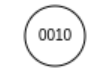
\includegraphics[width=.4\linewidth]{hp001}
		\caption{Elemento inicial 10.}
		\label{fig:sfig1}
	\end{subfigure}
	\begin{subfigure}{.3\textwidth}
		\centering
		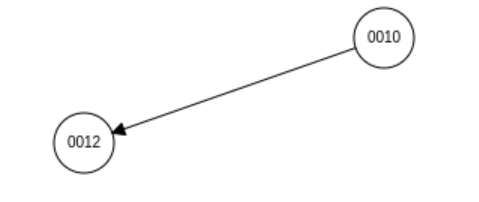
\includegraphics[width=1.4\linewidth]{hp002}
		\caption{Se agrega 12 y como es mayor solo se agrega como hoja.}
		\label{fig:sfig2}
	\end{subfigure}
	\begin{subfigure}{.3\textwidth}
		\centering
		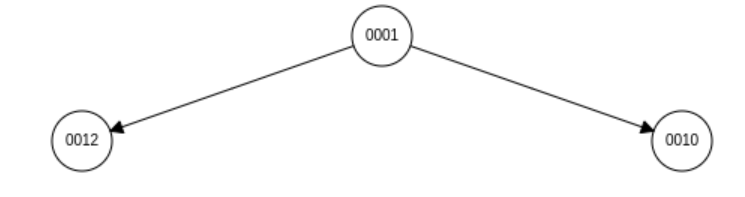
\includegraphics[width=1.8\linewidth]{hp003}
		\caption{1 es menor que todos los elementos así que se agrega como hoja, pero sube hasta la raíz.}
		\label{fig:sfig3}
	\end{subfigure}
	\begin{subfigure}{.6\textwidth}
		\centering
		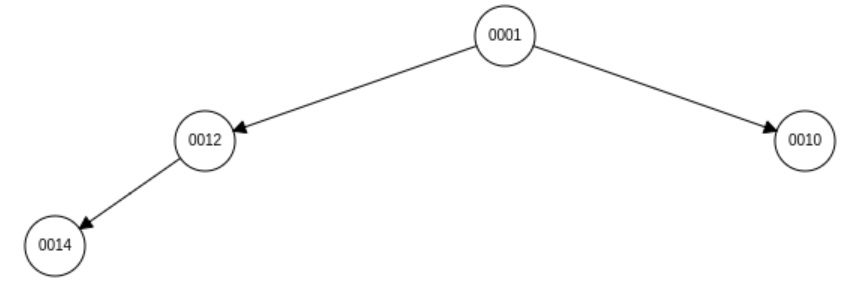
\includegraphics[width=1.04\linewidth]{hp004}
		\caption{14 es mayor que todos los otros elementos, se agrega como hoja.}
		\label{fig:sfig4}
	\end{subfigure}
	\begin{subfigure}{.6\textwidth}
		\centering
		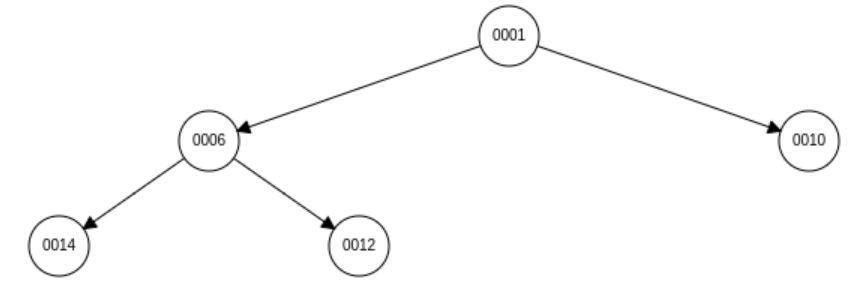
\includegraphics[width=1.04\linewidth]{hp005}
		\caption{6 se agrega como hoja pero es menor a 12, así que sube.}
		\label{fig:sfig5}
	\end{subfigure}
\begin{subfigure}{.6\textwidth}
	\centering
	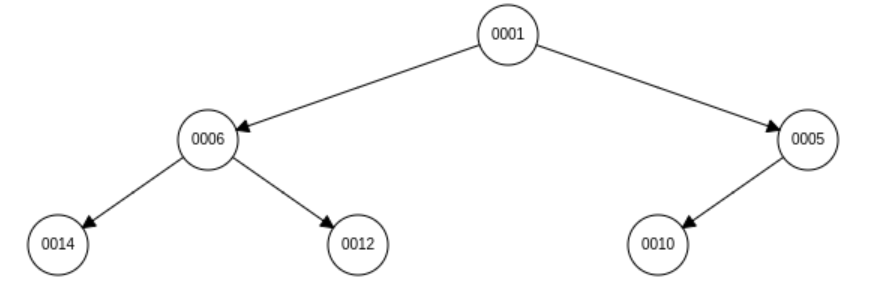
\includegraphics[width=1.04\linewidth]{hp006}
	\caption{Se agrega 5 como hoja pero es menor a 10 así que sube.}
	\label{fig:sfig6}
\end{subfigure}
\begin{subfigure}{.6\textwidth}
	\centering
	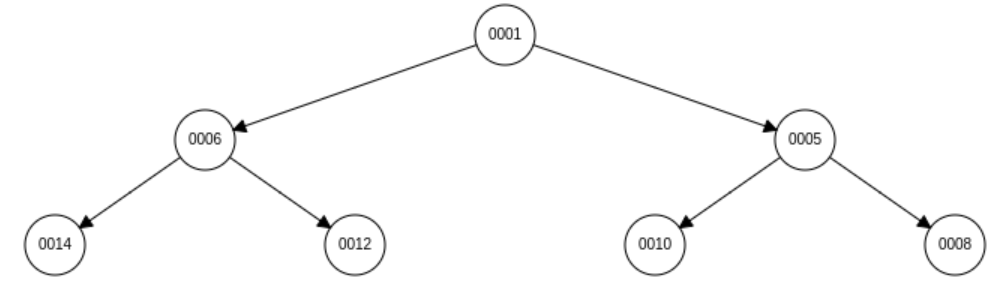
\includegraphics[width=1.04\linewidth]{hp007}
	\caption{Se agrega 8 como hoja y como es mayor a 5 se queda así.}
	\label{fig:sfig7}
\end{subfigure}
\begin{subfigure}{.6\textwidth}
	\centering
	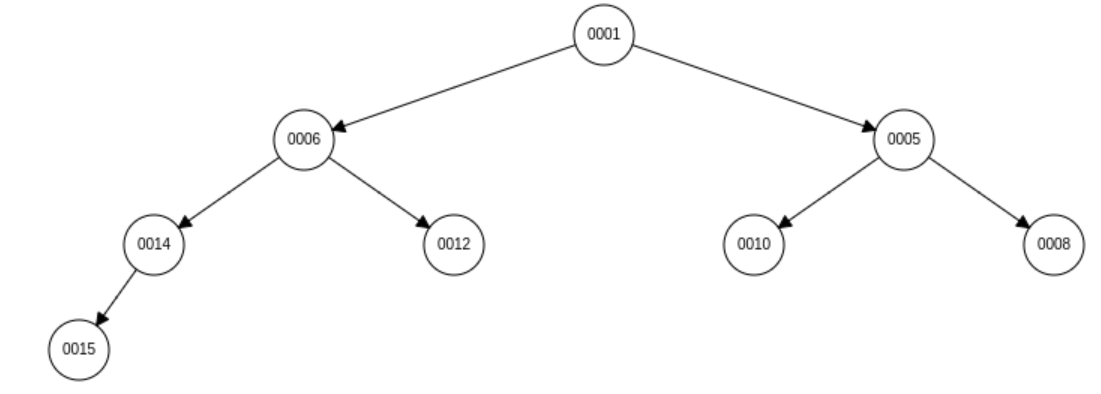
\includegraphics[width=0.95\linewidth]{hp008}
	\caption{Se agrega 15 como hoja y como es el mayor, se queda así.}
	\label{fig:sfig8}
\end{subfigure}
\begin{subfigure}{.6\textwidth}
	\centering
	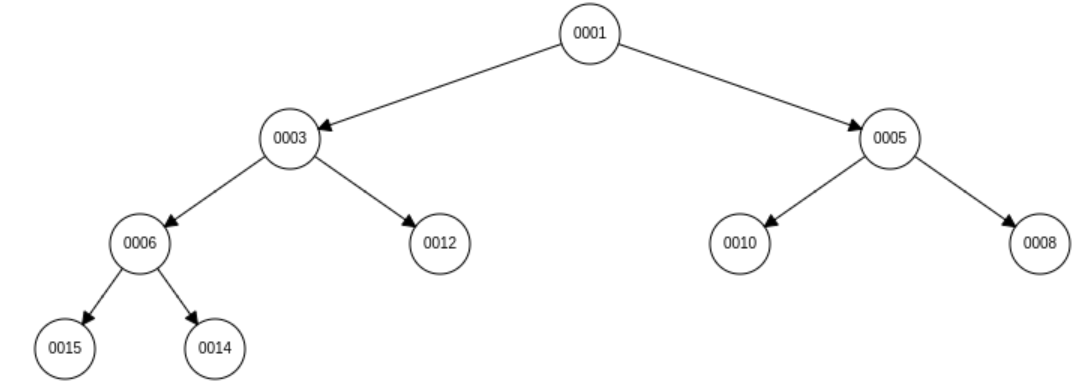
\includegraphics[width=1.04\linewidth]{hp009}
	\caption{Se agrega 3 como hoja y como es menor a 14 y a 6, sube dos niveles.}
	\label{fig:sfig9}
\end{subfigure}
	\caption{Árboles binarios en las primeras 9 inserciones.}
	\label{fig:fig}
\end{figure}
\begin{figure}
	\begin{subfigure}{.7\textwidth}
		\centering
		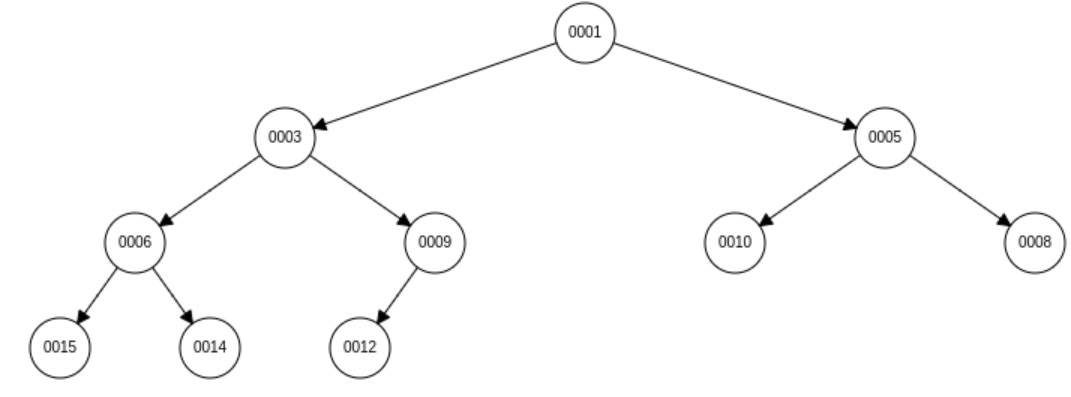
\includegraphics[width=1.1\linewidth]{hp010}
		\caption{Se agrega 9 como hoja y como es menor a 12, sube.}
		\label{fig:sfig10}
	\end{subfigure}
\begin{subfigure}{.7\textwidth}
	\centering
	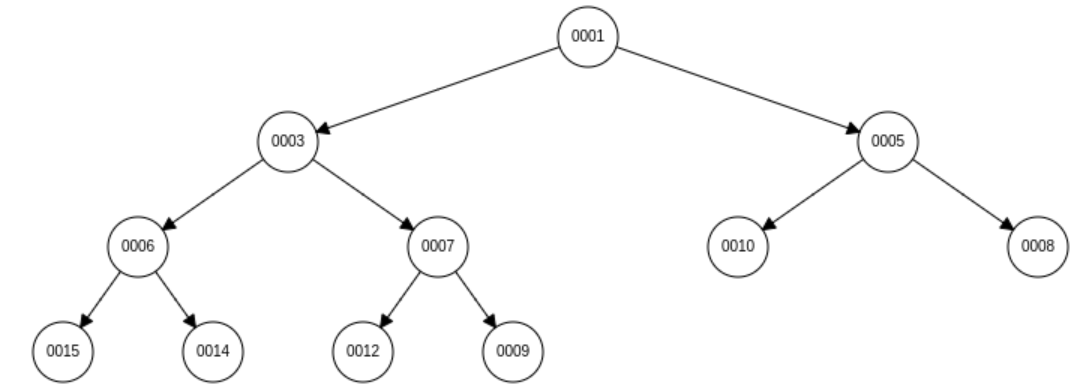
\includegraphics[width=1.1\linewidth]{hp011}
	\caption{Se agrega 7 como hoja y como es menor a 9, sube.}
	\label{fig:sfig11}
\end{subfigure}
\begin{subfigure}{.7\textwidth}
	\centering
	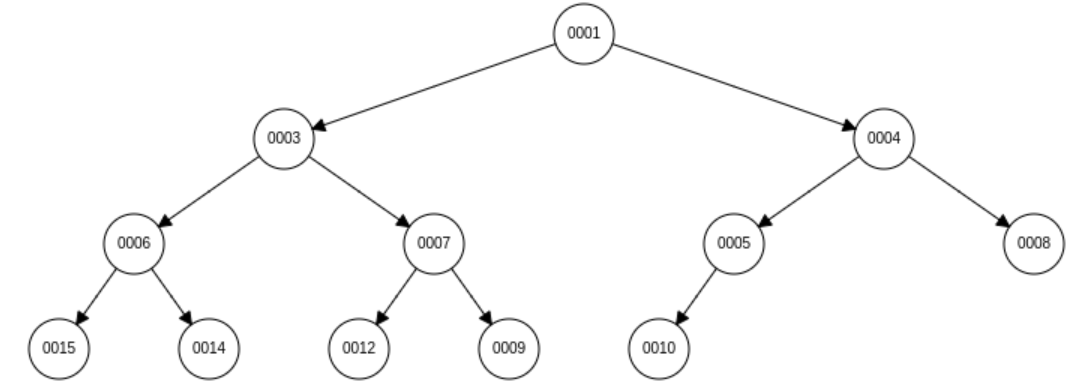
\includegraphics[width=1.1\linewidth]{hp012}
	\caption{Se agrega 4 como hoja y como es menor a 10 y 5, sube dos niveles.}
	\label{fig:sfig12}
\end{subfigure}
\begin{subfigure}{.7\textwidth}
	\centering
	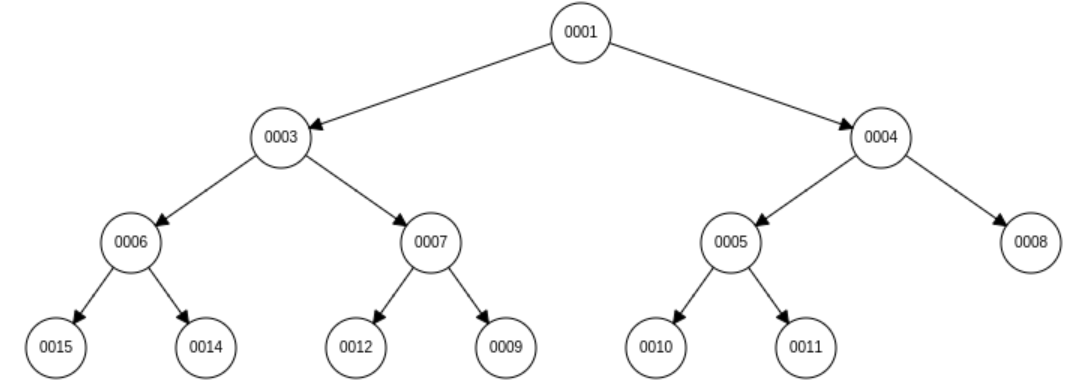
\includegraphics[width=1.1\linewidth]{hp013}
	\caption{Se agrega 11 como hoja y como es mayor a 5, se queda así}
	\label{fig:sfig13}
\end{subfigure}
	\caption{Árboles binarios en las siguientes 4 inserciones.}
	\label{fig:fig_}
\end{figure}
\begin{figure}
\begin{subfigure}{.9\textwidth}
	\centering
	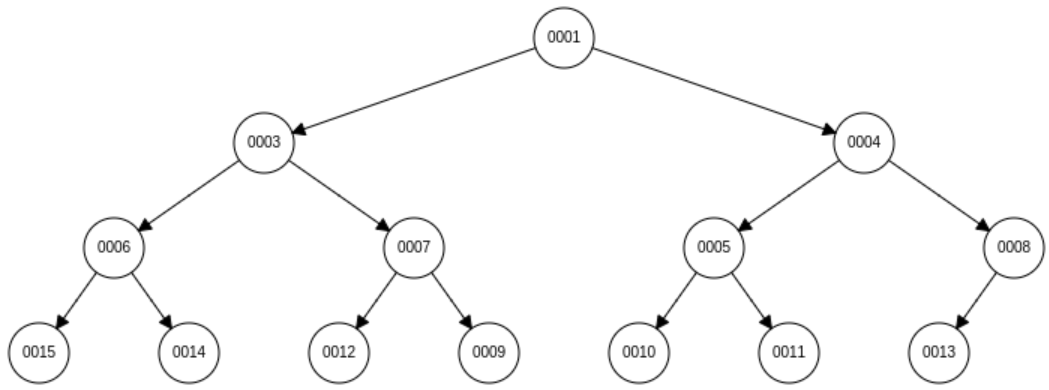
\includegraphics[width=1.2\linewidth]{hp014}
	\caption{Se agrega 13 y como es mayor a 8 así se queda. }
	\label{fig:sfig14}
\end{subfigure}
\begin{subfigure}{.9\textwidth}
	\centering
	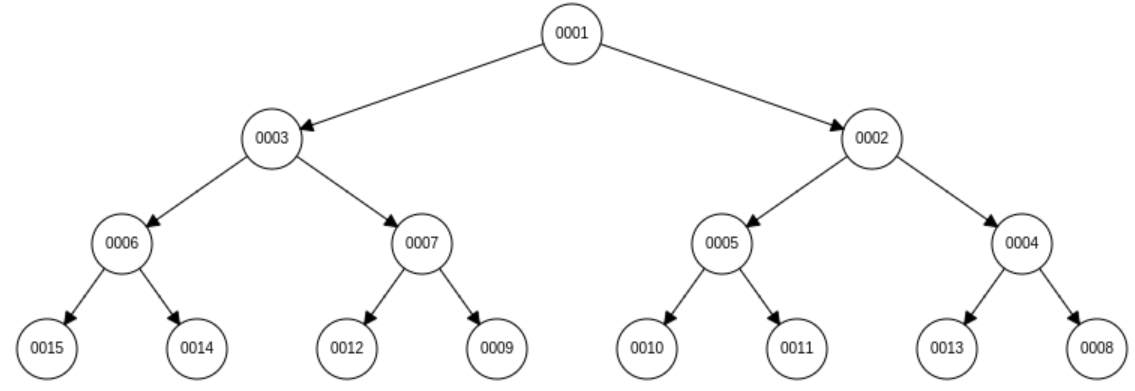
\includegraphics[width=1.2\linewidth]{hp015}
	\caption{Se agrega 2 como hoja y como es mayor a 8 y a 4, sube dos niveles.}
	\label{fig:sfig15}
\end{subfigure}
	\caption{Árboles binarios en las últimas 2 inserciones.}
	\label{fig:fig__}
\end{figure}
\pagebreak
\section{Ejercicio 5.}
\subsection{Demuestra en detalle y con una figura, por qué el algoritmo de Dijkstra es correcto.}
 \paragraph{}
	\begin{algorithm}[H]\footnotesize
	\KwResult{Calcular las distancias mínimas para todos los nodos $v$ de una gráfica $G$  a partir de un nodo $s \in G$.}
	\SetAlgoLined
	Inicializar $d(v):=infinito$, para toda $v \in G$\;
	Asignar $d(s):=0$\;
	Inicializar el conjunto de nodos $S:=\{s\}$\;
	\While{exista un nodo $v\notin S$ y que tenga una arista desde algún nodo $u\in S$}{
		Escogemos el nodo $v$ tal que  $v\notin S$ y que tenga una arista desde algún nodo $u\in S$
		y que tenga la mínima estimación de distancia, es decir que minimice: $d(u) + peso_{(u, v)}$\;
		\tcc{Es la suma entre la distancia mínima de $u$ mas el peso de la arista que conecta $u$ y a $v$.}
		 \tcp{Ahora, asignamos la mínima estimación de distancia  a $v$.}
		$d(v):=d(u) + peso_{(u, v)}$\;
		Agregamos $v$ al conjunto $S$\;
	}
	\caption{Dijkstra.}
\end{algorithm}
\begin{figure}[h]
	\begin{center}
	\begin{tikzpicture}[roundbknode/.style={draw,shape=circle,fill=black!40,minimum size=1mm}, roundbunode/.style={draw,shape=circle,fill=blue!40,minimum size=1mm}]
	\tikz
	%Nodes
	\node[roundbunode,label={north west:$v_1$}]      (s)                     {};
	\node[label={...}, color=orange]      (v2)       [above right=of v1] {};
	\node[label={$...$}]      (v3)       [below right=of v1] {};
	\node[roundbunode,label={north east:$u$}]      (v4)       [right=of v3] {};
	\node[roundbunode,label={north:$x$}]      (v5)       [right=of v2] {};
	\node[roundbknode,label={north east:$v$}]      (v6)       [right=of v4] {};
	\node[roundbknode,label={north east:$y$}]      (v7)       [right=of v5] {};
	%Lines
	\draw[color=orange, ->] (v1) -- (v2) node[midway,above] {};
	\draw[->] (v1) -- (v3) node[midway,below] {};
	\draw[->] (v3) -- (v4) node[midway,below] {};
	\draw[color=orange, ->] (v2) -- (v5) node[midway,below] {};
	\draw[->] (v4) -- (v6) node[midway,below] {};
	\draw[color=orange, ->] (v5) -- (v7) node[midway,below] {$e$};
	\draw[color=orange, dashed, ->] (v7) -- (v6) node[midway, right] {$P'$};
	\end{tikzpicture}
	\caption{Gráfica demo, con nodos del conjunto $S$ en color azul.}
	\label{fig4}
\end{center}
\end{figure}
\paragraph{Demostración de que el algoritmo termina.}
El algoritmo ejecuta cada iteración si existe algún nodo $v$ sin explorar y que tiene una arista desde $u$, que es un nodo en $S$ y ya esta explorado. En cada iteración al nodo $v$ con mínima estimación de distancia se agrega al conjunto $S$ y no vuelve a ser considerado en la siguiente iteración. Por lo tanto en cuanto todos los nodos estén en $S$ o no puedan ser explorados desde algún nodo en $S$ terminaran las iteraciones. Como a lo mas todos los nodos pueden ser explorados desde el nodo $s$, existirán a lo más $n - 1$ iteraciones del ciclo en la línea 4.
 \paragraph{Demostración de correctitud.} Por inducción:\\
 \textbf{Invariante:} Si el nodo $u$ esta en el conjunto $S$, entonces $d(u)$ es la mínima distancia desde $s$ a $u$.\\
  \textbf{Caso Base:} $|S|=1$, al iniciar el algoritmo $S=\{s\}$ y $d(s) =0$, lo cual es correcto.\\
  \textbf{Hipótesis Inductiva:} Asumir verdadero para $|S|\geq 1$.\\
  Sea $v$ el siguiente nodo a ser agregado a $S$, eso quiere decir que su estimación de distancia fue la mínima, es decir que la distancia del nodo  $u\in S$ que llega a $v$ mas el peso de la arista $(u,v)$ es menor o igual a cualquier otra distancia de un nodo $x\in S$ mas el peso de su arista a cualquier otro nodo $y\notin S$.\\
  Le sigue que mostremos que esta estimación de distancia es de hecho la distancia mínima desde $s$ a $v$. Como se muestra en la figura \ref{fig4} el camino con las aristas en negritas es el camino actual a $v$ que pasa por $u$, este es el camino mínimo pues de existir otro camino $P'$, que en la figura esta de color naranja, tiene que pasar por algún nodo $x\in S$. En el momento de agregar $v$ a $S$, $x$ fue revisado en la iteración pero su distancia mas el peso de su arista a cualquier otro nodo $y\notin S$ no fue menor a la estimación de $v$, pues se escogió la estimación de $v$ como la mínima. Al no existir otro camino con una estimación de distancia estrictamente menor, entonces al ser agregado algún nodo $v$ a $S$,  $d(v)$ es la mínima distancia entre $s$ y $v$.
 \section{Ejercicio 6}
 \subsection{Ofrece un algoritmo que, dada una cola de prioridad implementada con heaps binarios y con $n$ elementos, elimine el elemento $i$-ésimo de la cola. Analiza su complejidad y demuestra que en efecto tu algoritmo es correcto y tiene la complejidad que presumes.}
 \paragraph{} 
 \begin{algorithm}[H]
 	\SetAlgoLined
 	\KwData{Índice $i$ del elemento a eliminar}
		Asignamos el nuevo valor en $i$ como el menor valor entre el del hijo izquierdo y el hijo derecho, o VACÍO$\backslash$NULL (Lo eliminamos) en caso de que no tenga ningún hijo.\;
 		\eIf{tiene hijo izquierdo y el valor del hijo izquierdo fue el menor}{
 				llamar REMOVER($indice\_hijo\_izquierdo$)\;
 		}{
 		\If{tiene hijo derecho y el valor del hijo derecho fue el menor}{
 			llamar REMOVER($indice\_hijo\_derecho$)\;
 		}
 	}
 	\caption{Algoritmo REMOVER para eliminar el elemento $i$-ésimo de la cola de prioridad}
 \end{algorithm}
\paragraph{Complejidad} El algoritmo en cada llamada solo realiza una comparación entre los valores entre los hijos en el heap binario del $i$-ésimo elemento, y selecciona el menor entre los dos, o el valor único si solo tiene un hijo, o VACÍO$\backslash$NULL si no tiene hijos, que es el caso que el elemento a eliminar es una hoja y no habrá quien lo reemplace. La comparación y revisiones para ver si tiene hijos dentro de una llamada podemos considerarlas como operaciones constantes, sin embargo se multiplicará por el número de llamadas. Cada llamada recursiva se realiza si el elemento en el índice $i$ a remover tiene al menos un hijo, y se realiza una llamada en el hijo izquierdo o derecho. Entonces el número de llamadas corresponde a la cantidad de niveles en el heap binario a partir del índice $i$. En el peor de los casos donde el elemento a remover es la raíz y se recorren todos los niveles del heap binario se habrían hecho $log_2(n)$ llamadas pues es la altura de un heap binario balanceado de $n$ elementos.\\ Finalmente se tendría que con $log_2(n)$ llamadas y con operaciones constantes se tendría una complejidad de orden $O(log_2(n))$.
\paragraph{Correctitud} El algoritmo termina pues en el análisis de complejidad se llega que a lo más se realizarían $log_2(n)$ llamadas y una serie de operaciones constantes en cada llamada.\\
Ahora al terminar el algoritmo termina con un heap binario $A$ con los mismos elementos con excepción del elemento que se eliminó y estaba en la posición $i$. Lo que hace el algoritmo es reemplazar ese elemento con el menor de sus hijos si tiene alguno. La relación del padre de $i$ con $i$ es: \\
$A[padre(i)] \leq A[i]$\\
Y la relación de $i$ con sus hijos es:\\
$A[i] \leq A[hijo\_izq(i)]$ y  $A[i] \leq A[hijo\_der(i)]$\\
Entonces se cumple que:\\
$A[padre(i)] \leq A[hijo\_der(i)]$ y $A[padre(i)] \leq A[hijo\_izq(i)]$\\
Así que las invariantes de las  relaciones de orden se mantienen al reemplazar el valor en $i$ con alguno de sus hijos, y ahora al seleccionar al menor de ambos se cumplirá recursivamente a sus hijos.
Por lo tanto el orden en el heap binario se mantiene hasta llegar a una hoja y no quede mas que colocar un valor NULL. Finalmente se o termina con un heap binario $A$ con los mismos elementos con excepción del elemento que se eliminó y estaba en la posición $i$.
\pagebreak
\section{Ejercicio 7.}
\subsection{Sea $G=(V,E)$ una gráfica. Demuestra que cualesquiera dos de las siguientes propiedades implican la tercera.}
\begin{enumerate}
	\item $G$ es conexa.
	\item $G$ no tiene ciclos.
	\item $|E| = |V| - 1$.
\end{enumerate}
\paragraph{Demostremos que $1$ y $3$ implican $2$.}
Supongamos a $G$ una gráfica que cumple con $1$, y $3$. La gráfica $G$ tiene $n$ nodos, es decir $|V| = n$. En un ciclo de $z$ nodos se requieren $z$ aristas, pues para que el camino que comprende al ciclo se complete el último nodo debe tener una arista al primero, así los $z$ nodos tienen una arista. Pero solo tenemos $n - 1$ aristas por la propiedad $3$, la única forma de tener un ciclo es conectando una cantidad $x<n$ de nodos con $x$ aristas, pero dejarán sin arista a algún nodo, dejándolo  desconectado, pero eso no es posible por la propiedad $1$. Finalmente no es posible formar un ciclo en $G$ manteniendo $|V| - 1$ aristas y manteniendo a $G$ conexo.
\paragraph{Demostremos que $2$ y $3$ implican $1$.}
Supongamos a $G$ una gráfica que cumple con $1$, y $3$. Dejemos desconectado a por lo menos un nodo $u$ de $G$, eso nos dejaría con $n-1$ nodos conectados con $n-1$ aristas. Ahora en esos $n-1$ nodos para estar conectados, todos los nodos deben tener al menos una arista que lo conecte a otro de los $n-1$ nodos, como tienen $n-1$ aristas, es una arista para cada uno. Le sigue que como es conexo si exploramos desde uno de esos $n-1$ nodos llegaremos a todos los otros $n-1$ nodos, pues en nuestra suposición inicial $u$ es el único nodo desconectado. Pero al llegar al nodo $n-1$ en el camino, ese nodo también tiene una arista que nos llevará a otro de los $n-1$ nodos que ya exploramos, siendo entonces un ciclo. Por lo tanto si tenemos $n-1$ aristas y $n$ nodos, no podemos evitar tener un ciclo al dejar al menos un nodo desconectado. Finalmente si tenemos $n-1$ aristas y no tenemos ciclos entonces $G$ es conexa.
\pagebreak
\paragraph{Demostremos que $1$ y $2$ implican $3$.}
Supongamos a $G$ una gráfica que cumple con $1$, y $2$. Tomando en cuenta las observaciones de la demostración anterior, sabemos que si tenemos $n$ nodos conectados y $n$ aristas tendremos un ciclo. Así pues debemos tener menos que $n$ aristas para evitar formar un ciclo al ser conexa la gráfica. Probemos que podemos construir una gráfica conexa con $n$ nodos con $n-1$ aristas para cualquier $n>1$. Caso para $n=1$, con un solo nodo, es conexa con $0$ aristas. Ahora para  construir cualquier otra gráfica conexa podemos agregar un nuevo nodo con una nueva arista a ese nodo inicial o a cualquier otro nodo que pueda llegar al nodo inicial. Cualquier gráfica conexa que construyamos de esa forma  tendrá $n-1$ aristas, pues con cada nodo nuevo se agrega una arista, con excepción del nodo inicial. Probemos que no podemos construir una gráfica conexa con menos de $n-1$ aristas, el valor mas grande que es menor a $n-1$ es $n-2$. Si tomamos el caso con $n=2$ tendremos 0 aristas, dejando 2 nodos desconectados, y agregando una arista nueva y un nodo nuevo para $n>2$ dejará al menos un nodo desconectado.\\
Por lo tanto si debemos tener menos que $n$ aristas para evitar tener ciclos, no podemos tener menos de $n-2$ aristas pues dejaría de ser conexa, y con $n-1$ aristas si podemos tener  formar una gráfica conexa llegamos a que solo podemos tener $n-1$ aristas.
\section{Ejercicio 8.}
\subsection{El resumen se anexa al final del documento para cumplir con las especificaciones de formato.}
\pagebreak
\section{Ejercicio 9.}
\subsection{Para resolver el problema del cálculo de distancias entre todos los vértices de una gráfica dirigida $G=(V,E)$ con pesos en las aristas positivos o negativos, se pueden utilizar los siguientes algoritmos con respectivas complejidades:}
 \begin{itemize}
\item Algoritmo de Ford $O(|V|^{2}|E|)$
\item Algoritmo de Floyd $O(|V|^{3})$
\item Algoritmo de Johnson $O(|V|^{2}log(|V|) + |V| \cdot |E|)$ 
 \end{itemize}
Determina qué algoritmo conviene usar como función de $|E|$.
\paragraph{} Si el comportamiento de las funciones serán analizadas en función de $|E|$, es útil revisar el caso cuando $|E|$ tiene el mayor valor posible con $|V|$ nodos. El mayor valor es $\frac{|V|\cdot(|V| - 1)}{2}$ el cual es un valor cercano a $|V|^{2}$, cabe mencionar que en gráficas dirigidas donde la arista $(u, v)$ no necesariamente es igual a la arista $(v, u)$ y tenga aristas de la forma $(u, u)$, el valor será directamente $|V|^{2}$, entonces las complejidades para cada algoritmo serán cercanas a:\\
 \begin{itemize}
	\item Algoritmo de Ford $\approx O(|V|^{2}\cdot|V|^{2}) \approx O(|V|^{4})$
	\item Algoritmo de Floyd $O(|V|^{3})$
	\item Algoritmo de Johnson $\approx O(|V|^{2}log(|V|) + |V| \cdot|V|^{2}) \approx O(|V|^{2}log|V| + |V|^{3}) \approx O(|V|^{3})$ 
\end{itemize}
Es útil revisar el caso cuando $|E|$ tiene el menor valor posible con $|V|$ nodos. Como no hay restricciones de ser conexa $G$ el valor de $|E|$ puede ser $0$, entonces las complejidades para cada algoritmo serán cercanas a:\\
\begin{itemize}
	\item Algoritmo de Ford $\approx O(|V|^{2}\cdot 0) \approx O(1)$
	\item Algoritmo de Floyd $O(|V|^{3})$
	\item Algoritmo de Johnson $\approx O(|V|^{2}log(|V|) + |V| \cdot0) \approx O(|V|^{2}log|V|)$
\end{itemize}
Revisemos el caso cuando $|E| = |V|$, entonces las complejidades para cada algoritmo serán cercanas a:\\
\begin{itemize}
	\item Algoritmo de Ford $\approx O(|V|^{2}\cdot |V|) \approx O(|V|^{3})$
	\item Algoritmo de Floyd $O(|V|^{3})$
	\item Algoritmo de Johnson $\approx O(|V|^{2}log(|V|) + |V| \cdot|V|) \approx O(|V|^{2}log|V| + |V|^{2})$
\end{itemize}
El algoritmo que mas conviene en función de $|E|$ es el algoritmo de Johnson pues no importa que tan grande pueda ser $|E|$, el algoritmo tendrá como complejidad aproximada $O(|V|^{3})$ que es igual a Floyd y menor a Ford. Además de que si ahora consideramos menores valores de $|E|$ el algoritmo de Johnson tiene la mejor función de complejidad entre los 3, es decir para todos los valores de $|E|$ que cumplan $|V|^{2} > |E| \geq |V|$. En los únicos valores donde conviene usar a Ford en vez de Johnson es para valores de $|E|$ que cumplan $log(|V|) > |E| \geq 0$, pues Johnson no baja de $O(|V|^{2}log(|V|))$ aún con $|E| = 0$.
\section{Ejercicio 10.}
\subsection{Prueba que agregar una constante a todos los pesos y que multiplicar por una constante positiva no altera el conjunto de árboles generadores mínimos de una gráfica conexa con pesos dada.}
\paragraph{Demostración} Tomemos a cualquier árbol generador $MST_x$ de una gráfica $G$ con $n$ nodos, no necesariamente mínimo, y revisemos el cálculo de su peso total:
\begin{equation}
peso\_original(MST_x) = \sum_{i=1}^{n - 1} peso\_arista_i 
\end{equation}
La ecuación se refiere a que el peso total de cualquier árbol generador $MST_x$  es la suma de los pesos de las aristas que lo componen.\\
Ahora tomemos la primera transformación que es agregar una constante a todos los pesos. La ecuación 1 queda:
\begin{equation}
\begin{split}
peso\_suma\_constante(MST_x) & = \sum_{i=1}^{n - 1} (peso\_arista_i + C ) \\
&\quad = (\sum_{i=1}^{n - 1} peso\_arista_i) + (\sum_{i=1}^{n - 1} C) \\  
&\quad = (\sum_{i=1}^{n - 1} peso\_arista_i) + [(\sum_{i=1}^{n - 1}1) \cdot C] \\  
&\quad = (\sum_{i=1}^{n - 1} peso\_arista_i) + [(n-1) \cdot C] \\  
&\quad = peso\_original(MST_x)+ [(n-1) \cdot C] \\  
\end{split}
\end{equation}
En la ecuación 2 podemos ver que al agregar una constante a todos los pesos,  al valor $peso\_original(MST_x)$ solo se le agrega $[(n-1) \cdot C]$. Esto no afecta ninguna relación de orden entre este $MST_x$ y cualquier otro $MST_y$ pues como se agregó la constante a todos los pesos, cualquier otro $MST_y$ habrá aumentado su peso con la misma constante $[(n-1) \cdot C]$, manteniendo su orden relativo.\\
Ahora tomemos la segunda transformación que es multiplicar por una constante positiva a todos los pesos. La ecuación 1 queda:
\begin{equation}
\begin{split}
peso\_multiplica\_constante(MST_x) & = \sum_{i=1}^{n - 1} (peso\_arista_i \cdot C ) \\
&\quad = (\sum_{i=1}^{n - 1} peso\_arista_i) \cdot (C) \\  
&\quad = peso\_original(MST_x) \cdot C\\  
\end{split}
\end{equation}
En la ecuación 3 podemos ver que al multiplicar por una constante positiva a todos los pesos, el valor $peso\_original(MST_x)$ solo se incrementa en un factor de $C$. Esto no afecta ninguna relación de orden entre este $MST_x$ y cualquier otro $MST_y$ pues como se multiplicó por una constante positiva a todos los pesos, cualquier otro $MST_y$ habrá aumentado su peso en un factor de la misma constante $C$, manteniendo su orden relativo.\\
Finalmente como ninguna de las transformaciones modifica el orden que existe entre los árboles generadores, entonces no afecta el conjunto de los árboles generadores mínimos, ya que se mantienen siendo mínimos en comparación a los demás árboles generadores y por las demostraciones anteriores ese orden no se altera.\\
\section{Ejercicio 11.}
\subsection{Demuestra que si todas las aristas de una gráfica conexa $G$ tienen pesos diferentes dos a dos, entonces $G$ tiene un sólo árbol generador mínimo.}
\paragraph{Demostración} Por contradicción\\
Supongamos que hay mas de un árbol generador mínimo, es decir tenemos al menos 2 árboles distintos. Supongamos que dichos árboles son $MST_1$ y $MST_2$. Esos dos árboles son distintos y por lo tanto hay al menos una arista $e \in MST_1$ tal que $e\notin MST_2$ y de igual forma hay al menos una arista $e' \notin MST_1$ tal que $e'\in MST_2$.\\
Tomemos el caso de la  arista $e \in MST_1$ tal que $e\notin MST_2$, tomemos el cutset $C_1$ que corresponde al cutset donde la única arista que lo atraviesa es $e$, es decir que $e$ es la única arista que es miembro de $MST_1$ y además une un nodo $u\in S_a$ con un nodo $v\in S_b$,  siendo $S_a$ y $S_b$ los dos conjuntos de nodos del cutset $C_1$.\\
Ahora tomemos ese cutset pero desde $MST_2$ en este caso debe haber al menos una arista que lo atraviese, aunque también puede haber mas de una. Le sigue que la arista $e$ del $MST_1$ es distinta a cualquiera de estas aristas en el $MST_2$. Por lo tanto tienen peso mayor al peso de la arista $e$, o un peso menor.\\ Tomemos el caso que alguna de esas aristas $e'$ tiene peso menor que $e$, eso significa que en el $MST_1$ podemos reemplazar a $e$ con $e'$ pues $e'$ conecta el mismo cutset. Sin embargo como $e'$ tiene peso menor significa que el peso total del $MST_1$ disminuiría, pero esto es una contradicción pues $MST_1$ ya tenía peso mínimo. Por lo tanto no existe dicha arista $e'$ que es menor a $e$ para ese cutset. Tomemos entonces el caso que esas aristas en $MST_2$ para el cutset $C_1$ son mayores. Eso significa que pasa lo inverso, que $MST_2$ puede reemplazar cualquiera de esas aristas por $e$ y así disminuir el peso total de $MST_2$, sin embargo eso también es una contradicción pues $MST_2$ ya era de peso mínimo. Por lo tanto no pueden existir aristas distintas a $e$ en $MST_2$  para el cutset $C_1$. Como no pueden existir esas aristas entonces no puede haber ni una sola arista $e\in MST_1$ tal que $e\notin MST_2$. Finalmente significa que no puede existir mas de un único árbol generador mínimo para una gráfica $G$ donde todas las aristas tienen pesos diferentes dos a dos.
\section{Ejercicio 12.}
\subsection{Dado un árbol generador mínimo de una gráfica con pesos $G=(V,E)$ supongamos que una arista de $G$ es eliminada sin desconectar la gráfica. Describe cómo encontrar un nuevo árbol recubridor mínimo en tiempo proporcional a $|E|$.}
Al remover la arista pueden pasar dos casos:
\begin{enumerate}
\item La arista eliminada no pertenecía al árbol generador mínimo.
\item La arista eliminada pertenecía al árbol generador mínimo.
\end{enumerate}
Para el primer caso, el nuevo árbol generador mínimo sería el mismo con que el árbol original.
Para el segundo caso, al perder una arista del árbol generador mínimo terminamos con dos conjuntos de nodos $S_a$ y $S_b$, podemos explorar dichos conjuntos para poder 'etiquetarlos' y poder saber a cuál de los dos conjuntos pertenece algún nodo. Dicha exploración se hace en tiempo proporcional a $|V|$ puesto que como son árboles ambos conjuntos de nodos, a lo mas se recorren $|S_a|-1 + |S_b|-1$ aristas, y como $|S_a| + |S_b| = |V|$, se recorren a lo mas $|V|-2$ aristas.\\ 
Ya con los nodos 'etiquetados', podemos recorrer el conjunto de aristas $E$, y si esa arista no es parte del árbol recubridor y ademas conecta un nodo en $S_a$ y a un nodo en $S_b$ lo guardamos como posible respuesta. Al considerar nuevas posibles respuestas nos vamos quedando con la menor. Con esa arista y las otras aristas que no fueron eliminadas del árbol recubridor mínimo original podemos formar nuestro nuevo árbol recubridor mínimo. Este proceso fue de tiempo $|E|$ pues recorrimos todas las aristas, sin importar el orden, solo que mantenemos a la menor que encontremos.
\section{Ejercicio 13.}
\subsection{Diseña un algoritmo que resuelva el siguiente problema y demuestra que tiene la complejidad que se solicita: dada una gráfica conexa $G$ con pesos positivos, encontrar en a lo más tiempo $O(mlog(m))$, un árbol recubridor mínimo que minimice la arista más costosa.}
\paragraph{Observación.} Se utilizará el algoritmo de Kruskal para obtener un árbol generador de peso mínimo. Posterior a demostrar la correctitud y complejidad para esta tarea, se demostrará que el árbol generador de peso mínimo resultante, sea $MST$, es también un árbol generador tal que no existe otro árbol generador (no necesariamente mínimo) que tenga una arista máxima menor a la arista máxima de $MST$.\\
\begin{algorithm}[H]\footnotesize
	\KwResult{Un árbol generador mínimo.}
	\KwIn{Una Gráfica $G=(V,E)$}
	\SetAlgoLined
	Ordenar todas las aristas $e \in E$ de menor a mayor peso\;
	\tcp{Inicializar el valor de padre a cada nodo}
	$padre[u]=u$ para todo $u\in V$\;
	\tcp{Inicializar el tamaño del conjunto de cada nodo}
	$tamano[u]=1$ para todo $u\in V$\;
	\tcp{Inicializar el conjunto de aristas del árbol generador resultante.}
	$MST = \{\}$\;
	\ForEach{arista $(u,v, peso)\in E$}{
		\If{FIND($u$) != FIND($v$)}{ 
			UNION($u$, $v$)\;
			agregar arista $(u,v, peso)$ a $MST$\;
		}
	}
	\caption{Kruskal.}
\end{algorithm}
\begin{algorithm}[H]\footnotesize
	\KwResult{El padre de un conjunto.}
	\KwIn{Un nodo $u$}
	\SetAlgoLined
	\If{padre[$u$] != $u$}{ 
		return FIND(padre[u])\;
	}
	return $u$\;
	\caption{FIND.}
\end{algorithm}
\begin{algorithm}[H]\footnotesize
	\KwResult{Unir el conjunto que pertenece el nodo $u$ con el conjunto al que pertenece el nodo $v$.}
	\KwIn{Un nodo $u$ y un nodo $v$}
	\SetAlgoLined
	\eIf{tamano[FIND($u$)] $<$ tamano[FIND($v$)]}{ 
		padre[FIND($u$)] := FIND($v$)\;
		tamano[FIND($v$)] := tamano[FIND($v$)] + tamano[FIND($u$)];
	} {
	padre[FIND($v$)] := FIND($u$)\;
	tamano[FIND($u$)] := tamano[FIND($u$)] + tamano[FIND($v$)];
	}
	\caption{UNION.}
\end{algorithm}
\subsection{Demostraremos el algoritmo 6 para la operación UNION.}
\paragraph{El algoritmo termina y es de complejidad $O(1)$} El algoritmo solo realiza dos asignaciones, si el menor en tamaño es el conjunto al que pertenece $u$, se marca como nuevo padre del conjunto al padre del conjunto al que pertenece $v$, y sumando sus tamaños. En caso de que $v$ sea menor o igual se hacen las asignación pero intercambiando $u$ por $v$. Podemos considerar las asignaciones como operaciones constantes así la complejidad de una llamada de UNION será de orden $O(1)$.
\paragraph{El algoritmo asigna como padre del conjunto menor al padre del conjunto mayor.}
El algoritmo realiza dichas operaciones correspondientes posteriormente de hacer la comparación de tamaños en la linea 1.
\subsection{Demostremos el algoritmo 5 para la operación FIND.}
\paragraph{El algoritmo termina y tiene complejidad $O(log(n))$} El algoritmo seguirá llamando a FIND hasta que un nodo sea el mismo que el padre del conjunto al que pertenece. Inicialmente todos son el padre del conjunto al que pertenecen por la linea 2 en el algoritmo 4. El valor de padre[$u$] solo es modificado en la operación UNION, sin embargo solo cambia para uno de los dos nodos que recibe UNION. Por lo tanto uno de los dos se mantendrá. Le sigue que el padre de un conjunto $p$ siempre cumplirá que $padre[p] = p$. La cantidad de llamadas que realiza FIND corresponde a la cantidad de operaciones UNION hubo para formar al conjunto del que estamos buscando su padre. Esta cantidad no puede ser mayor a $log(n)$, esto pues para cada operación UNION se cambió el padre del conjunto más pequeño de $x$ elementos, esto es que el conjunto mayor tuvo al menos $x$ elementos, dejando un conjunto resultante de al menos $2x$ elementos. Ahora si este mismo conjunto cambió su padre significa que hubo otro conjunto de al menos $2x$ elementos y dejando un conjunto resultante de al menos $4x$ elementos. Así pues llegamos a que si la suma total de elementos es $n$, y cada cambió de padre multiplica en al menos 2 el número de elementos, no pudo haber más de $log(n)$ cambios de padre en un conjunto dado. Posteriormente tenemos que se hacen a lo más $log(n)$ llamadas a FIND. Finalmente como en cada llamada solo se realiza una comparación que consideramos constante $O(1)$, FIND tiene como complejidad $O(log(n))$.
\paragraph{El algoritmo regresa al padre del conjunto al que pertenece el nodo $u$}
El algoritmo no para hasta encontrarlo y solo revisa que en efecto el padre del conjunto es el mismo nodo $u$ y lo regresamos en la linea 4. Seguimos buscando en caso contrario y en la demostración anterior determinamos que llegará eventualmente al elemento padre del conjunto.
\subsection{Demostremos el algoritmo 4 para encontrar un árbol generador mínimo.}
\paragraph{El algoritmo termina}
Por la invariante de recorremos una sola vez cada arista en $E$ en el ciclo de la línea 5, a lo mas tendremos $|E|$ iteraciones.
\paragraph{El algoritmo es de complejidad $O(mlog(m))$}
El ordenar las aristas en la línea 1 ya es de $O(mlog(m))$. Ahora, el ciclo en la línea 5 también es $O(mlog(m))$, esto es porque se el ciclo tiene $m$ iteraciones y se realizan 2 operaciones FIND y una operación UNION, vimos en las demostraciones anteriores que FIND tiene una complejidad de $O(log(n))$ y UNION una complejidad de $O(1)$. Finalmente tenemos $O(mlog(m) + mlog(n))$, sin embargo como $m>=n-1$ el factor dominante es $mlog(m)$. Finalmente es de orden $O(mlog(m))$ como se solicita en el ejercicio.
\paragraph{Correctitud: El algoritmo regresa un árbol generador de peso mínimo.}
Por inducción.\\
\textbf{Invariante: } Si una arista esta en el conjunto resultante $MST$, dicha arista pertenece al árbol generador de peso mínimo.\\
\textbf{Caso base:} El conjunto $MST$ tiene a la primer arista del conjunto ordenado $E$, eso es que es la mínima arista para los nodos $u$ y $v$ que conecta la arista. Ese es el árbol generador mínimo para 2 nodos siendo estos $u$ y $v$, ya que por estar ordenados cualquier otra arista que los una y no es la primera tendrá peso mayor o igual a la primera.\\
\textbf{Hipótesis inductiva:} La siguiente arista que una dos conjuntos disjuntos será miembro del árbol generador mínimo.
Suponer verdadero hasta la $i$-ésima arista en agregar a $MST$.\\
Dicha arista $i$ une dos conjuntos disjuntos, pues esto se verifica antes de tomar la arista en la línea 6 del algoritmo 4. Sean $A$ y $B$ dichos conjuntos. Eso significa que podemos tomar el cutset $C_x$ que separa dos conjuntos de nodos, sean $S_a$ y $S_b$, tal que $A\subseteq S_a$ y $B\subseteq S_b$. Como el conjunto de aristas esta ordenada, la invariante es la arista $i$ es menor o igual a cualquier otra arista que este después de ella.\\
Por lo tanto cualquier otra arista que una al cutset $C_x$ y se encuentre después de $i$ tendrá peso mayor o igual a la arista $i$. Posteriormente, como esto se repetirá para los siguientes conjuntos disjuntos que una alguna arista posterior a $i$, podemos decir que para todo cutset para el cuál haya una sola arista en $MST$ que lo atraviese (pues se unieron dos conjuntos disjuntos) será siempre de peso mínimo. Finalmente como habrá $n-1$ aristas en $MST$ tendremos $n-1$ cutsets para los que tendremos aristas de peso mínimo que unieron conjuntos disjuntos de nodos, es decir que tendremos $n-1$ aristas que terminan conectando $n$ nodos, siendo esta la definición de un árbol generador de peso mínimo. 
\subsection{Demostración de que un árbol generador de peso mínimo es un árbol que minimiza un arista máxima.}
Por contradicción.\\
Supongamos que tenemos a nuestro árbol generador de peso mínimo $MST_1$ y que existe al menos un árbol generador $MST_2$ tal que su arista de mayor peso es menor a la arista de mayor peso en $MST_1$. Sea $e$ la arista de mayor peso en $MST_1$. Entonces la arista $e$ tiene peso estrictamente mayor al peso de toda arista que pertenece a $MST_2$.\\
Tomemos el cutset $C_1$ que corresponde al cutset donde la única arista que lo atraviesa es $e$, es decir que $e$ es la única arista que es miembro de $MST_1$ y además une un nodo $u\in S_a$ con un nodo $v\in S_b$, siendo $S_a$ y $S_b$ los dos conjuntos de nodos del cutset $C_1$.\\
Ahora tomemos ese cutset pero desde $MST_2$ en este caso debe haber al menos una arista que lo atraviese, aunque también puede haber mas de una. Le sigue que el peso de la arista $e$ del $MST_1$ es mayor al peso de cualquiera de estas aristas del $MST_2$. Sea $e'$ cualquiera de estas aristas del $MST_2$. Eso significa que en el $MST_1$ podemos reemplazar a $e$ con $e'$, pues $e'$ conecta el mismo cutset que conectaba $e$. Sin embargo como $e'$ tiene peso menor significa que el peso total del $MST_1$ disminuiría, pero esto es una contradicción pues $MST_1$ ya tenía peso mínimo. Por lo tanto no existe dicha arista $e'$ que es menor a $e$ para ese cutset. Como no pueden existir esas aristas entonces no puede haber ni una sola arista $e\in MST_1$ tal que sea de peso mayor a toda arista que pertenece a $MST_2$. Por lo tanto no puede existir ni un solo árbol generador tal que su arista de mayor peso es menor a la arista de mayor peso en $MST_1$. Finalmente un árbol generador de peso mínimo es también un árbol generador que minimiza su arista máxima.

\end{document}